% PlotNeuralNet rendering of the physics-constrained autoencoder.
% Faithful reproduction of the authors' diagram, with two changes:
%   (1) the leftmost node is the input spectrum image (SHO_input.png);
%   (2) the decoder equation is the manuscript's Eq.(1) (eq:sho), not the
%       malformed workshop expression.
\begin{tikzpicture}
\tikzstyle{connection}=[ultra thick,every node/.style={sloped,allow upside down},draw=\edgecolor,opacity=0.7]
\tikzstyle{copyconnection}=[ultra thick,every node/.style={sloped,allow upside down},draw={rgb:blue,4;red,1;green,1;black,3},opacity=0.7]

% ---------------------------------------------------------------------
% Input spectrum image (real & imaginary cantilever response).
% ---------------------------------------------------------------------
\node[canvas is zy plane at x=0, transform shape] (input) at (-3.4,0,0)
    {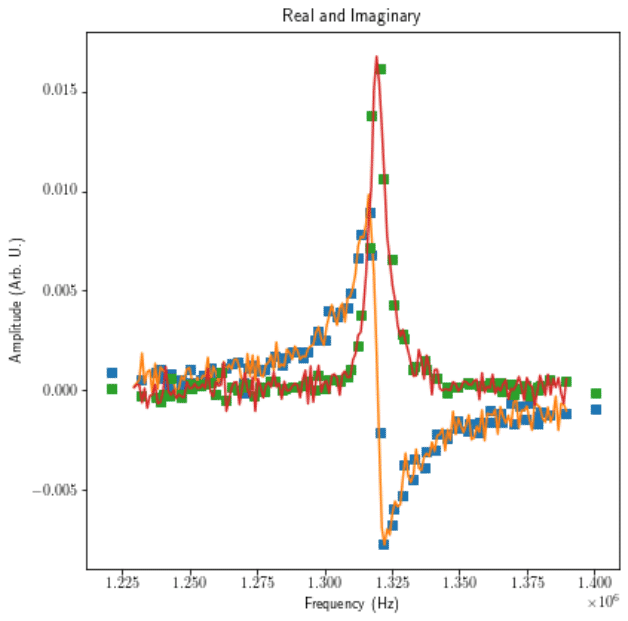
\includegraphics[width=8.5cm]{SHO_input.png}};
\node[below=2.0cm of input, font=\Large] {\textbf{Input}};

% ---------------------------------------------------------------------
% Encoder: three shrinking Conv1D slabs.
% ---------------------------------------------------------------------
\pic[shift={(0,0,0)}] at (0,0,0)
    {Box={
        name=ccr_b1,
        caption=Conv1D,
        xlabel={{8, }},
        zlabel=159,
        fill=\ConvColor,
        height=30,
        width=4,
        depth=40
        }
    };

\pic[shift={(1,0,0)}] at (ccr_b1-east)
    {Box={
        name=ccr_b2,
        caption=Conv1D,
        xlabel={{6, }},
        zlabel=153,
        fill=\ConvColor,
        height=30,
        width=3,
        depth=40
        }
    };

\draw [connection]  (ccr_b1-east)    -- node {\midarrow} (ccr_b2-west);

\pic[shift={(1,0,0)}] at (ccr_b2-east)
    {Box={
        name=ccr_b3,
        caption=Conv1D,
        xlabel={{4, }},
        zlabel=149,
        fill=\ConvColor,
        height=30,
        width=2,
        depth=40
        }
    };

\draw [connection]  (ccr_b2-east)    -- node {\midarrow} (ccr_b3-west);

\pic[shift={ (1,0,0) }] at (ccr_b3-east)
    {Box={
        name=pool_b4,
        caption=MaxPooling1D,
        fill=\PoolColor,
        opacity=0.5,
        height=30,
        width=2,
        depth=20
        }
    };

\draw [connection]  (ccr_b3-east)    -- node {\midarrow} (pool_b4-west);

% ---------------------------------------------------------------------
% Three banded Conv1D (4,4) blocks.
% ---------------------------------------------------------------------
\pic[shift={ (3,0,0) }] at (pool_b4-east)
    {RightBandedBox={
        name=ccr_b5,
        caption=Conv1D,
        xlabel={{ 4, 4 }},
        zlabel=40,
        fill=\ConvColor,
        bandfill=\ConvReluColor,
        height=30,
        width={ 2 , 2 },
        depth=20
        }
    };

\draw [connection]  (pool_b4-east)    -- node {\midarrow} (ccr_b5-west);

\pic[shift={ (1,0,0) }] at (ccr_b5-east)
    {RightBandedBox={
        name=ccr_b6,
        caption=Conv1D,
        xlabel={{ 4, 4 }},
        zlabel=40,
        fill=\ConvColor,
        bandfill=\ConvReluColor,
        height=30,
        width={ 2 , 2 },
        depth=20
        }
    };

\draw [connection]  (ccr_b5-east)    -- node {\midarrow} (ccr_b6-west);

\pic[shift={ (1,0,0) }] at (ccr_b6-east)
    {RightBandedBox={
        name=ccr_b7,
        caption=Conv1D,
        xlabel={{ 4, 4 }},
        zlabel=40,
        fill=\ConvColor,
        bandfill=\ConvReluColor,
        height=30,
        width={ 2 , 2 },
        depth=20
        }
    };

\draw [connection]  (ccr_b6-east)    -- node {\midarrow} (ccr_b7-west);

\pic[shift={ (1,0,0) }] at (ccr_b7-east)
    {Box={
        name=pool_b8,
        caption=AvgPooling1D,
        fill=\PoolColor,
        opacity=0.5,
        height=30,
        width=2,
        depth=10
        }
    };

\draw [connection]  (ccr_b7-east)    -- node {\midarrow} (pool_b8-west);

\pic[shift={(3,0,0)}] at (pool_b8-east)
    {Box={
        name=ccr_b9,
        caption=Conv1D,
        xlabel={{2, }},
        zlabel=14,
        fill=\ConvColor,
        height=30,
        width=1,
        depth=10
        }
    };

\draw [connection]  (pool_b8-east)    -- node {\midarrow} (ccr_b9-west);

\pic[shift={ (3,0,0) }] at (ccr_b9-east)
    {Box={
        name=pool_b10,
        caption=AvgPooling1D,
        fill=\PoolColor,
        opacity=0.5,
        height=30,
        width=1,
        depth=5
        }
    };

\draw [connection]  (ccr_b9-east)    -- node {\midarrow} (pool_b10-west);

\pic[shift={(3,0,0)}] at (pool_b10-east)
    {Box={
        name=ccr_b11,
        caption=Conv1D,
        xlabel={{2, }},
        zlabel=6,
        fill=\ConvColor,
        height=30,
        width=1,
        depth=5
        }
    };

\draw [connection]  (pool_b10-east)    -- node {\midarrow} (ccr_b11-west);

\pic[shift={ (3,0,0) }] at (ccr_b11-east)
    {Box={
        name=pool_b12,
        caption=AvgPooling1D,
        fill=\PoolColor,
        opacity=0.5,
        height=30,
        width=1,
        depth=5
        }
    };

\draw [connection]  (ccr_b11-east)    -- node {\midarrow} (pool_b12-west);

% ---------------------------------------------------------------------
% Flatten layer (8 = 2 channels x 4).
% ---------------------------------------------------------------------
\pic[shift={(3,0,0)}] at (pool_b12-east)
    {Box={
        name=flatten_b13,
        caption=Flatten Layer,
        xlabel={{" ","dummy"}},
        zlabel=8,
        fill=\SoftmaxColor,
        opacity=0.8,
        height=5,
        width=2,
        depth=40
        }
    };

\draw [connection]  (pool_b12-east)    -- node {\midarrow} (flatten_b13-west);

% ---------------------------------------------------------------------
% Dense branch tapped off the third Conv1D.
% ---------------------------------------------------------------------
\pic[shift={ (5,0,12) }] at (ccr_b3-south)
    {Box={
        name=dense_b14,
        caption=Dense,
        fill=\UnpoolColor,
        opacity=0.5,
        height=15,
        width=4,
        depth=10
        }
    };

\pic[shift={ (1,0,0) }] at (dense_b14-east)
    {Box={
        name=dense_b15,
        caption=Dense,
        fill=\UnpoolColor,
        opacity=0.5,
        height=15,
        width=4,
        depth=10
        }
    };

\draw [connection]  (dense_b14-east)    -- node {\midarrow} (dense_b15-west);
\draw [connection]  (ccr_b3-east)    -- node {\midarrow} (dense_b14-west);

% ---------------------------------------------------------------------
% Concat ball merging the flatten and dense paths.
% ---------------------------------------------------------------------
\pic[shift={(10,0,20)}] at (flatten_b13-east)
    {Ball={
        name=concat_b16,
        fill=\SumColor,
        opacity=0.6,
        radius=3,
        logo=$\cup$
        }
    };

\draw [connection]  (dense_b15-east)    -- node {\midarrow} (concat_b16-west);
\draw [connection]  (flatten_b13-east)    -- node {\midarrow} (concat_b16-west);

% ---------------------------------------------------------------------
% Dense taper to the latent (SHO parameters).
% ---------------------------------------------------------------------
\pic[shift={ (2,0,0) }] at (concat_b16-east)
    {Box={
        name=dense_b17,
        caption=Dense,
        fill=\UnpoolColor,
        opacity=0.5,
        height=12,
        width=4,
        depth=8
        }
    };

\pic[shift={ (2,0,0) }] at (dense_b17-east)
    {Box={
        name=dense_b18,
        caption=Dense,
        fill=\UnpoolColor,
        opacity=0.5,
        height=6,
        width=4,
        depth=4
        }
    };

\pic[shift={ (2,0,0) }] at (dense_b18-east)
    {Box={
        name=dense_b19,
        caption=Dense,
        fill=\UnpoolColor,
        opacity=0.5,
        height=3,
        width=4,
        depth=2
        }
    };

\draw [connection]  (concat_b16-east)    -- node {\midarrow} (dense_b17-west);
\draw [connection]  (dense_b17-east)    -- node {\midarrow} (dense_b18-west);
\draw [connection]  (dense_b18-east)    -- node {\midarrow} (dense_b19-west);

% ---------------------------------------------------------------------
% Boxed SHO decoder equation = manuscript Eq.(1) (eq:sho).
% ---------------------------------------------------------------------
\node[draw=black, very thin, fill=white, fill opacity=0.6, text opacity=1,
      rounded corners=2pt, inner sep=10pt, anchor=west]
      (sho) at (40,-3,0)
    {$\displaystyle \chi(\omega) =
        \frac{A\,\omega_0^{2}\,e^{i\phi}\,Q}
             {Q\,\omega^{2} - i\,\omega\,\omega_0 - Q\,\omega_0^{2}}$};

\draw[dashed]
    (dense_b19-nearnortheast) -- (sho.north west)
    (dense_b19-nearsoutheast) -- (sho.south west);

\end{tikzpicture}
